\section{Forward Sampling Strategies}
\label{sec:forwardSamplingStrategies}
In order to perform UQ and dynamic
probabilistic risk assessment (DPRA),
a sampling strategy needs to be employed. The sampling strategy
perturbs the input space (domain of the uncertainties) to explore
the response of a complex system in relation to selected FOMs.

The most widely used strategies to perform UQ and PRA are generally
collected in RAVEN as \textit{\textbf{Forward}} samplers. \textit{\textbf{Forward}} samplers include
all the strategies that simply perform the sampling of the input space.  These strategies sample
without exploiting, through learning approaches,
the information made available from the outcomes of evaluation previously performed (adaptive sampling) and the
common system evolution (patterns) that different sampled calculations can generate in the phase space (Dynamic Event Tree).

As mentioned in Section~\ref{sub:tutorialMultiRun}, RAVEN has
several different \textit{\textbf{Forward}} samplers:
\begin{itemize}
  \item \textit{Monte-Carlo}
  \item \textit{Grid-based}
  \item \textit{Stratified} and its specialization named \textit{Latin Hyper Cube}.
\end{itemize}
In addition, RAVEN posses advanced \textit{\textbf{Forward}} sampling strategies that:
\begin{itemize}
  \item Build a grid in the input space selecting evaluation points
    based on characteristic quadratures as part of stochastic collocation
    for generalized polynomial chaos method (\textit{Sparse
    Grid Collocation} sampler);
  \item Use high-density model reduction (HDMR) a.k.a. Sobol
    decomposition to approximate a function as the sum of
    interactions with increasing complexity (\textit{Sobol} sampler).
\end{itemize}
In the following subsections, we provide examples of input files
in RAVEN using the method, with explanatory commentary.
%%%%%%%%%%%%%%%%%%%%%%%%%
%%%%%%%%  MONTE-CARLO %%%%%%%%
%%%%%%%%%%%%%%%%%%%%%%%%%
\subsection{Monte-Carlo sampling through RAVEN}
\label{sub:MCexample}
The Monte-Carlo method is one of the most-used methodologies in several mathematic disciplines. In this section,
we will explain the techniques for employing this methodology in RAVEN, and we recommend the user to read the
theory manual to explore the theory of the method.
The goals of this section are about learning how to:
 \begin{enumerate}
   \item Set up a simple Monte-Carlo sampling for perturbing the input space of a driven code
   \item Load the outputs of the code into RAVEN DataObjects (HistorySets and PointSets)
   \item Print the contents of DataObjects to file
   \item Generate plots of the sampling results.
\end{enumerate}
In order to accomplish these tasks, the following RAVEN \textbf{Entities} (XML blocks in the RAVEN input file) are needed:
\begin{enumerate}
   \item \textbf{\textit{RunInfo}}:
     \xmlExample{framework/user_guide/ForwardSamplingStrategies/forwardSamplingMontecarlo.xml}{RunInfo}
     As discussed in Section~\ref{sub:singleRun}, the \textit{RunInfo} \textbf{Entity} sets up the analysis
     that the user wants to perform. The number of steps specified in (\xmlNode{Sequence}) are sequentially run using the number of processors assigned in (\xmlNode{batchSize}). 
     Note that the \xmlNode{JobName} is not required, but is useful in identifying the input file.
   \item \textbf{\textit{Models}}:
     \xmlExample{framework/user_guide/ForwardSamplingStrategies/forwardSamplingMontecarlo.xml}{Models}
     The Model used in this example is the \textbf{Projectile} external model, which is defined in section \ref{sec:analyticalbateman}.  
   \item \textbf{\textit{Distributions}}:
     \xmlExample{framework/user_guide/ForwardSamplingStrategies/forwardSamplingMontecarlo.xml}{Distributions}
     In the \xmlNode{Distributions} block, the stochastic model for the uncertainties treated by the
     \xmlNode{Sampler} is defined. In this case two distributions are defined:
  \begin{itemize}
    \item $vel\_dist \sim \mathbb{N}(30,5)$, used to model the uncertainties
    associated with  the \textit{velocity};
    \item  $angle\_dist \sim \mathbb{U}(5,85)$,  used to
    model the uncertainties associated with the \textit{angle}.
  \end{itemize}
   \item \textbf{\textit{Samplers}}:
     \xmlExample{framework/user_guide/ForwardSamplingStrategies/forwardSamplingMontecarlo.xml}{Samplers}
      To employ the Monte-Carlo sampling strategy, a
      \xmlNode{MonteCarlo} node needs to be defined. The number of samples is defined within this node. The Monte-Carlo method is employed on model variables listed by name and are associated with a distribution.
   \item \textbf{\textit{DataObjects}}:
     \xmlExample{framework/user_guide/ForwardSamplingStrategies/forwardSamplingMontecarlo.xml}{DataObjects}
      In this block, three \textit{DataObjects} are defined to store results: 1) a PointSet named
      ``samples'', 2) a PointSet named ``dummyIN'' 3) a HistorySet named ``histories''.
      Note that in the \xmlNode{Input} node all the uncertainties
      perturbed through the Monte-Carlo strategy are listed. By this, any
      realization in the input space is linked in the DataObject to the outputs listed in the
      \xmlNode{Output} node. Furthermore, since we use an external model that does not have any input file, we define a pointset named ``dummyIN'' that is used as a dummy input in the multirun step.
   \item \textbf{\textit{OutStreams}}:
     \xmlExample{framework/user_guide/ForwardSamplingStrategies/forwardSamplingMontecarlo.xml}{OutStreams}
 %%%%%%%%%%%%%%%%%%%%%%%%%%%%%%%%%%%%%%%%%%%%%%%%%%%%%%%%%%
 %figure histories
 \begin{figure}[h!]
  \centering
  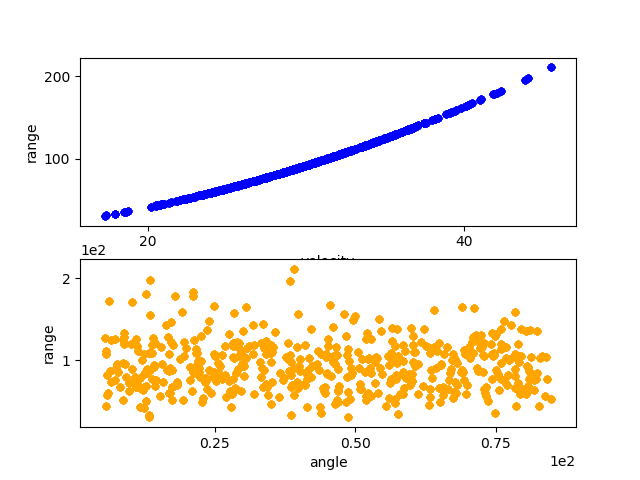
\includegraphics[scale=0.7]{../../tests/framework/user_guide/ForwardSamplingStrategies/gold/RunDir/MonteCarlo/1-historyPlot_scatter-scatter.png}
  \caption{Plot of the histories generated by the Monte Carlo sampling.}
  \label{fig:historiesMCPlotScatter}
 \end{figure}
 %%%%%%%%%%%%%%%%%%%%%%%%%%%%%%%%%%%%%%%%%%%%%%%%%%%%%%%%%%
 To see the results of the simulation, \xmlNode{OutStreams} are included in the input.
  In this block, both OutStream types are used:
  \begin{itemize}
    \item \textit{Print}:
     \begin{itemize}
       \item ``samples'' connected with the \textit{DataObjects} \textbf{Entity} ``samples''
                (\xmlNode{source})
       \item ``histories'' connected with the \textit{DataObjects} \textbf{Entity} ``histories'' (\xmlNode{source})
     \end{itemize}
     Note that in RAVEN, multiple entities can have the same name, as it takes a class, a type, and a name to uniquely identify a RAVEN object. When the two OutStream objects are used, all the information contained in the  linked \textit{DataObjects} are going
    to be exported in CSV files (\xmlNode{type}).
    \item \textit{Plot}:
    \begin{itemize}
      \item ``historiesPlot'' connected with the  \textit{DataObjects}
      \textbf{Entity} ``histories''.  This plot shows the variable $range$ with respect to the input variables $velocity$ and $angle$.
      \item ``samplesPlot3D'' connected with the
      \textit{DataObjects} \textbf{Entity} ``samples''. This plot shows the variables $range,time$ with respect to the input variables $velocity$ and $angle$.
    \end{itemize}
     Note that both plots use gridded subplots. Two plots
     are placed in each of the figures.
  \end{itemize}
   \item \textbf{\textit{Steps}}:
     \xmlExample{framework/user_guide/ForwardSamplingStrategies/forwardSamplingMontecarlo.xml}{Steps}
 %%%%%%%%%%%%%%%%%%%%%%%%%%%%%%%%%%%%%%%%%%%%%%%%%%%%%%%%%%
 %figure samples
 \begin{figure}[h!]
  \centering
  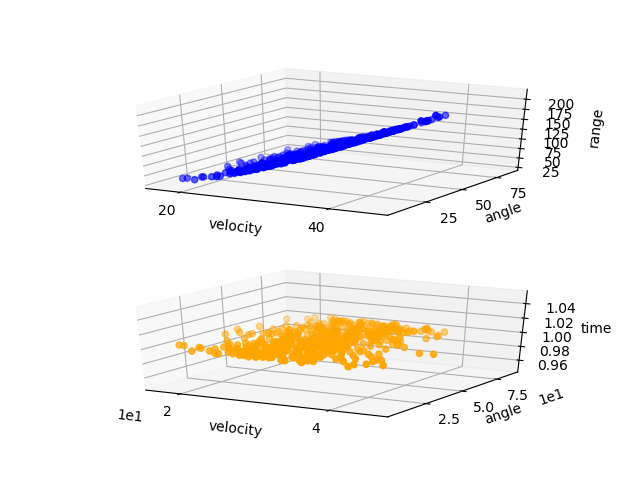
\includegraphics[scale=0.7]{../../tests/framework/user_guide/ForwardSamplingStrategies/gold/RunDir/MonteCarlo/1-samplesPlot3D_scatter-scatter.png}
  \caption{Plot of the samples generated by the MC sampling.}
  \label{fig:samplesMCPlotScatter}
 \end{figure}
 %%%%%%%%%%%%%%%%%%%%%%%%%%%%%%%%%%%%%%%%%%%%%%%%%%%%%%%%%%
   Once all the other entities are defined in the RAVEN input file, they must be combined in the
   \xmlNode{Steps} block, which dictates the workflow of RAVEN.  For this case,
   two \xmlNode{Steps} are defined:
   \begin{itemize}
     \item \xmlNode{MultiRun} ``sample'', used to run the multiple
     instances of the driven code and
     collect the outputs in the two \textit{DataObjects}. As it can be
     seen, the \xmlNode{Sampler} is specified to communicate to the
     \textit{Step} that the driven code needs to
     be perturbed through the Monte-Carlo sampling.
     \item  \xmlNode{IOStep} named ``writeHistories'', used to 1) dump
     the ``histories'' and ``samples'' \textit{DataObjects}
     \textbf{Entity} to a CSV file and 2) plot the data in the EPS file.
   \end{itemize}
\end{enumerate}
 Figures~\ref{fig:historiesMCPlotScatter} and ~\ref{fig:samplesMCPlotScatter} show the report
 generated by RAVEN.
%%%%%%%%%%%%%%%%%%%%%%%%%
%%%%%%%%          GRID          %%%%%%%%
%%%%%%%%%%%%%%%%%%%%%%%%%
\subsection{Grid sampling through RAVEN}
\label{sub:Gridexample}
The Grid sampling method (also known as Full Factorial Design of Experiment) represents one of the simplest methodologies that can be employed in order to explore the interaction of multiple random variables with respect
selected FOMs.
The goal of this section is to show how to:
 \begin{enumerate}
   \item Set up a simple Grid sampling for performing a parametric analysis of a driven code
   \item Load the outputs of the code into the RAVEN DataObjects system
   \item Print out what contained in the DataObjects
   \item Generate basic plots of the code result.
\end{enumerate}
In order to accomplish these tasks, the following RAVEN \textbf{Entities} (XML blocks in the input files) are required:
\begin{enumerate}
   \item \textbf{\textit{RunInfo}}:
     \xmlExample{framework/user_guide/ForwardSamplingStrategies/forwardSamplingGrid.xml}{RunInfo}
   As shown in Section~\ref{sub:singleRun}, the \textit{RunInfo} \textbf{Entity} is intended to set up the desired analysis. The number of steps specified in (\xmlNode{Sequence}) are sequentially run using the number of processors assigned in (\xmlNode{batchSize}). 
   \item \textbf{\textit{Models}}:
     \xmlExample{framework/user_guide/ForwardSamplingStrategies/forwardSamplingGrid.xml}{Models}
 The Model here is represented by the \textbf{Projectile}, which already dumps its output file in a
 CSV format (standard format that RAVEN can read). 
   \item \textbf{\textit{Distributions}}:
     \xmlExample{framework/user_guide/ForwardSamplingStrategies/forwardSamplingGrid.xml}{Distributions}
  In the Distributions XML section, the stochastic model for the
  uncertainties  treated by the Grid sampling are reported. In
  this case two distributions are defined:
  \begin{itemize}
    \item $vel\_dist \sim \mathbb{N}(30,5)$, used to model the uncertainties
    associated with  the \textit{velocity};
    \item  $angle\_dist \sim \mathbb{U}(5,85)$,  used to
    model the uncertainties associated with the \textit{angle}.
  \end{itemize}
   \item \textbf{\textit{Samplers}}:
     \xmlExample{framework/user_guide/ForwardSamplingStrategies/forwardSamplingGrid.xml}{Samplers}
  To employ the Grid sampling strategy, a
  \xmlNode{Grid} node needs to be specified. As shown above, in each variable section, the  \xmlNode{grid} is defined.
   \item \textbf{\textit{DataObjects}}:
     \xmlExample{framework/user_guide/ForwardSamplingStrategies/forwardSamplingGrid.xml}{DataObjects}
  In this block, three \textit{DataObjects} are defined to store results: 1) a PointSet named
      ``samples'', 2) a PointSet named ``dummyIN'' 3) a HistorySet named ``histories''.
  In the \xmlNode{Input} node all the variables  perturbed through the Grid strategy are listed. In this way, any  realization in the input space is linked to the outputs listed in  the
  \xmlNode{Output} node. As described earlier as well, since we use an external model that does not have any input file, we define a pointset named ``dummyIN'' that is used as a dummy input in the multirun step.
    \item \textbf{\textit{OutStreams}}:
     \xmlExample{framework/user_guide/ForwardSamplingStrategies/forwardSamplingGrid.xml}{OutStreams}
 %%%%%%%%%%%%%%%%%%%%%%%%%%%%%%%%%%%%%%%%%%%%%%%%%%%%%%%%%%
 %figure histories
 \begin{figure}[h!]
  \centering
  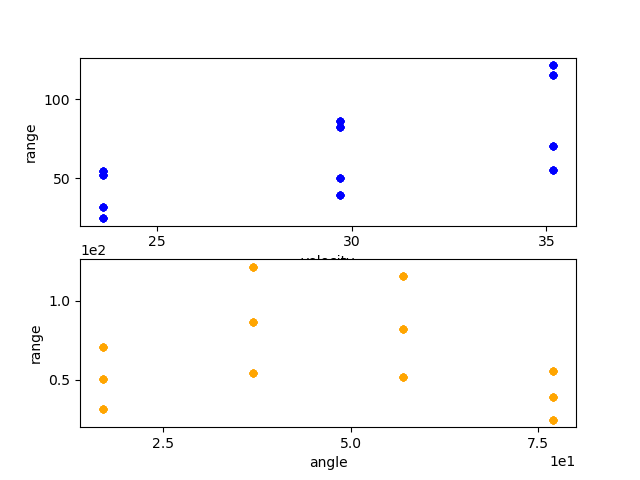
\includegraphics[scale=0.7]{../../tests/framework/user_guide/ForwardSamplingStrategies/gold/RunDir/Grid/1-historyPlot_scatter-scatter.png}
  \caption{Plot of the histories generated by the Grid sampling.}
  \label{fig:historiesGridPlotScatter}
 \end{figure}
 %%%%%%%%%%%%%%%%%%%%%%%%%%%%%%%%%%%%%%%%%%%%%%%%%%%%%%%%%%
  In this block, both the Out-Stream types are constructed:
  \begin{itemize}
    \item \textit{Print}:
     \begin{itemize}
       \item named ``samples'' connected with the \textit{DataObjects} \textbf{Entity} ``samples''
                (\xmlNode{source})
       \item named ``histories'' connected with the \textit{DataObjects} \textbf{Entity} ``histories'' (\xmlNode{source}).
     \end{itemize}
      When these objects get used, all the information contained in the
      linked  \textit{DataObjects} are going
    to be exported in CSV files (\xmlNode{type}).
    \item \textit{Plot}:
    \begin{itemize}
      \item named ``historiesPlot'' connected with the  \textit{DataObjects}
      \textbf{Entity} ``histories''.  This plot shows the variable $range$ with respect to the input variables $velocity$ and $angle$.
      \item named ``samplesPlot3D'' connected with the
      \textit{DataObjects} \textbf{Entity} ``samples''. This plot shows the variables $range,time$ with respect to the input variables $velocity$ and $angle$.
    \end{itemize}
  \end{itemize}
   \item \textbf{\textit{Steps}}:
     \xmlExample{framework/user_guide/ForwardSamplingStrategies/forwardSamplingGrid.xml}{Steps}
 %%%%%%%%%%%%%%%%%%%%%%%%%%%%%%%%%%%%%%%%%%%%%%%%%%%%%%%%%%
 %figure samples
 \begin{figure}[h!]
  \centering
  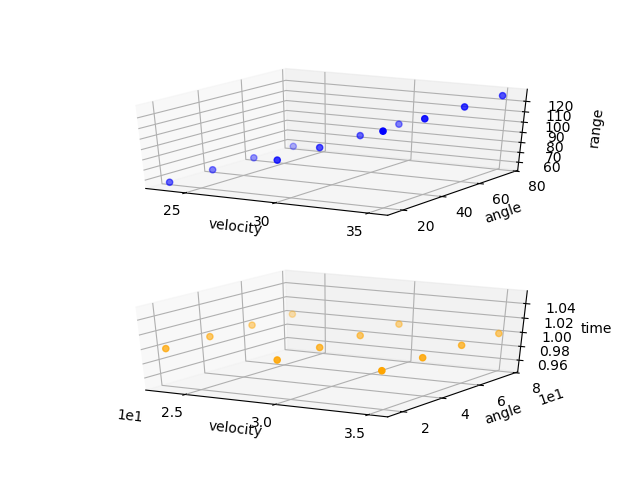
\includegraphics[scale=0.7]{../../tests/framework/user_guide/ForwardSamplingStrategies/gold/RunDir/Grid/1-samplesPlot3D_scatter-scatter.png}
  \caption{Plot of the samples generated by the Grid sampling for variables $A,B,C,D$.}
  \label{fig:samplesGridPlotScatter}
 \end{figure}
 %%%%%%%%%%%%%%%%%%%%%%%%%%%%%%%%%%%%%%%%%%%%%%%%%%%%%%%%%%
   Finally, all the previously defined \textbf{Entities} can be combined in
   the \xmlNode{Steps} block. As inferable,
   two \xmlNode{Steps} have been inputted:
   \begin{itemize}
     \item \xmlNode{MultiRun} named ``sample'', is used to run the multiple
     instances of the code and
     collect the outputs in the two \textit{DataObjects}. As it can be
     seen, the \xmlNode{Sampler} is inputted to communicate to the
     \textit{Step} that the driven code needs to
     be perturbed through the Grid sampling
     \item  \xmlNode{IOStep} named ``writeHistories'', used to 1) dump
     the ``histories'' and ``samples'' \textit{DataObjects}
     \textbf{Entity} in a CSV file and 2) plot the data in the PNG file and
     on the screen.
   \end{itemize}
\end{enumerate}
 Figures~\ref{fig:historiesGridPlotScatter} and ~\ref{fig:samplesGridPlotScatter} display the report generated by RAVEN.

%%%%%%%%%%%%%%%%%%%%%%%%%
%%%%%%%%    STRATIFIED    %%%%%%%%
%%%%%%%%%%%%%%%%%%%%%%%%%
\subsection{Stratified sampling through RAVEN}
\label{sub:Stratifiedexample}
The Stratified sampling is a class of methods that relies on the assumption that the input space (i.e.,uncertainties)
can be separated in regions (strata) based on similarity of the response of the system for input set within the
same strata. Following this assumption, the most rewarding (in terms of computational cost vs. knowledge gain)
sampling strategy would be to place one sample for each region. In this way, the same information is not
collected more than once and all the prototypical behavior are sampled at least once. In
Figure~\ref{fig:StratifiedSamplingExample}, the Stratified sampling approach is exemplified.
 \begin{figure}[h!]
  \centering
  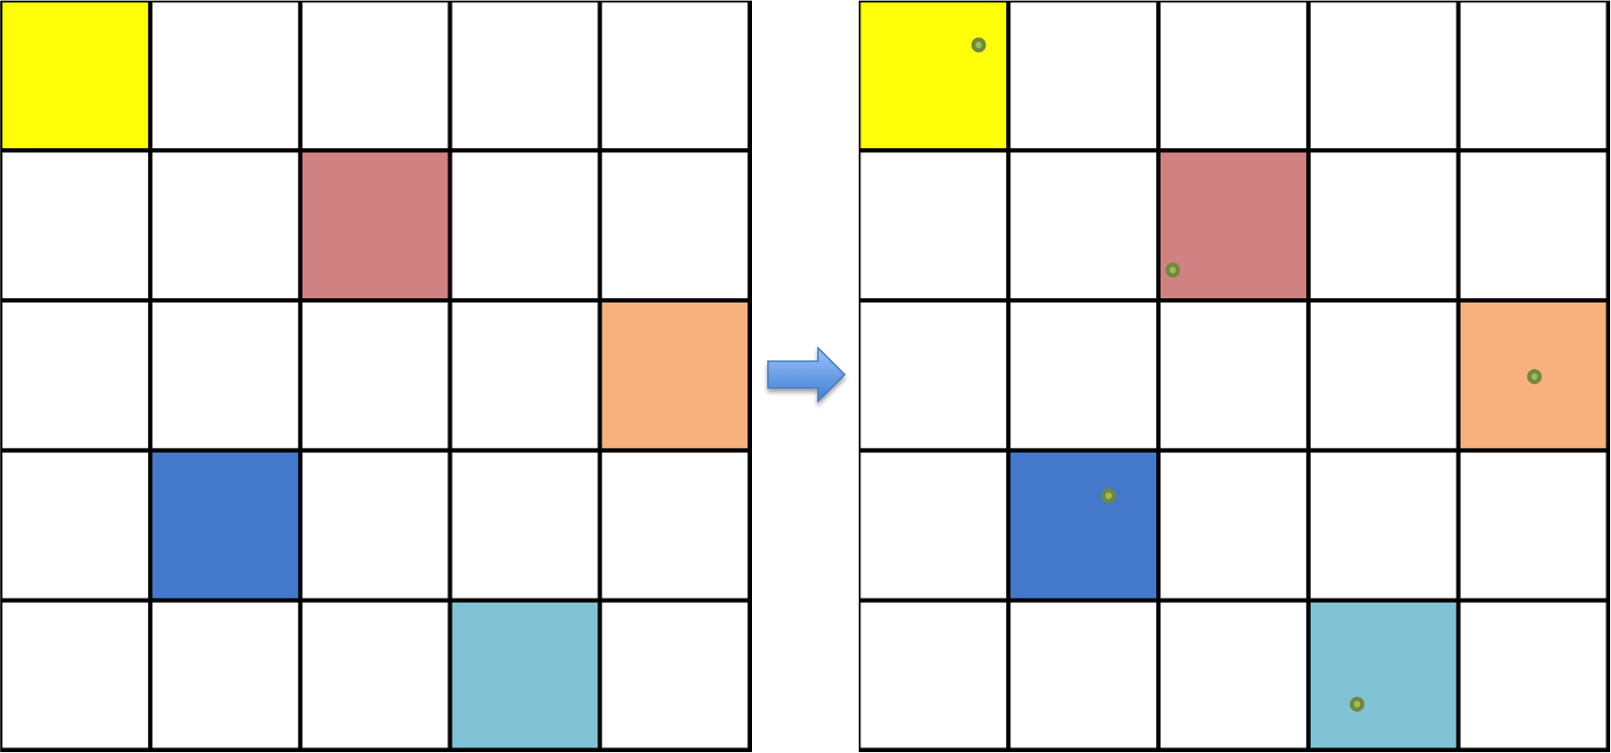
\includegraphics[scale=0.55]{pics/StratifiedSamplingExample.png}
  \caption{Example of Stratified sampling approach.}
  \label{fig:StratifiedSamplingExample}
 \end{figure}
\\The goal of this section is to show how to:
 \begin{enumerate}
   \item Set up a simple Stratified sampling in order to perform a parametric analysis on a driven code
   \item Load the outputs of the code into the RAVEN DataObjects system
   \item Print out what contained in the DataObjects
   \item Generate basic plots of the code result.
\end{enumerate}
To accomplish these tasks, the following RAVEN \textbf{Entities} (XML blocks in the input files) are defined:
\begin{enumerate}
   \item \textbf{\textit{RunInfo}}:
     \xmlExample{framework/user_guide/ForwardSamplingStrategies/forwardSamplingStratified.xml}{RunInfo}
   As explained earlier, the \textit{RunInfo} \textbf{Entity} is intended to set up the analysis that the user wants to perform. The number of steps specified in (\xmlNode{Sequence}) are sequentially run using the number of processors assigned in (\xmlNode{batchSize}).
   \item \textbf{\textit{Models}}:
     \xmlExample{framework/user_guide/ForwardSamplingStrategies/forwardSamplingStratified.xml}{Models}
 The Model here is represented by the
 \textbf{Projectile}, which already dumps its output file in a
 CSV format (standard format that RAVEN can read).
   \item \textbf{\textit{Distributions}}:
     \xmlExample{framework/user_guide/ForwardSamplingStrategies/forwardSamplingStratified.xml}{Distributions}
  In the Distributions XML section, the stochastic model for the
  uncertainties  treated by the Stratified sampling are reported. In
  this case two distributions are defined:
  \begin{itemize}
    \item $vel\_dist \sim \mathbb{N}(30,5)$, used to model the uncertainties
    associated with  the \textit{velocity};
    \item  $angle\_dist \sim \mathbb{U}(5,85)$,  used to
    model the uncertainties associated with the \textit{angle}.
  \end{itemize}
   \item \textbf{\textit{Samplers}}:
     \xmlExample{framework/user_guide/ForwardSamplingStrategies/forwardSamplingStratified.xml}{Samplers}
  To employ the Stratified sampling strategy, a
  \xmlNode{Stratified} node needs to be specified. In each variable section, the  \xmlNode{grid} is defined.
  It is important to mention that the number of \xmlAttr{steps} needs to be the same for each of the variables,  since, as reported in previous section, the Stratified sampling strategy it discretizes the domain in strata.
  The number of samples finally requested is equal to $n_{samples} = n_{steps} = 100$.
  If the grid for each variables is defined in CDF and of  \xmlAttr{type} = ``equal'', the Stratified sampling corresponds to the well-known Latin Hyper Cube sampling.
   \item \textbf{\textit{DataObjects}}:
     \xmlExample{framework/user_guide/ForwardSamplingStrategies/forwardSamplingStratified.xml}{DataObjects}
  In this block, two \textit{DataObjects} are defined: 1) a PointSet named
      ``samples'', 2) a PointSet named ``dummyIN'' 3) a HistorySet named ``histories''.
  In the \xmlNode{Input} node all the variables perturbed through the Stratified strategy are listed. In this way, any realization in the input space is linked to the outputs listed in  the
  \xmlNode{Output} node. Since we use an external model that does not have any input file, we define a pointset named ``dummyIN'' that is used as a dummy input in the multirun step.
   \item \textbf{\textit{OutStreams}}:
     \xmlExample{framework/user_guide/ForwardSamplingStrategies/forwardSamplingStratified.xml}{OutStreams}
 %%%%%%%%%%%%%%%%%%%%%%%%%%%%%%%%%%%%%%%%%%%%%%%%%%%%%%%%%%
 %figure histories
 \begin{figure}[h!]
  \centering
  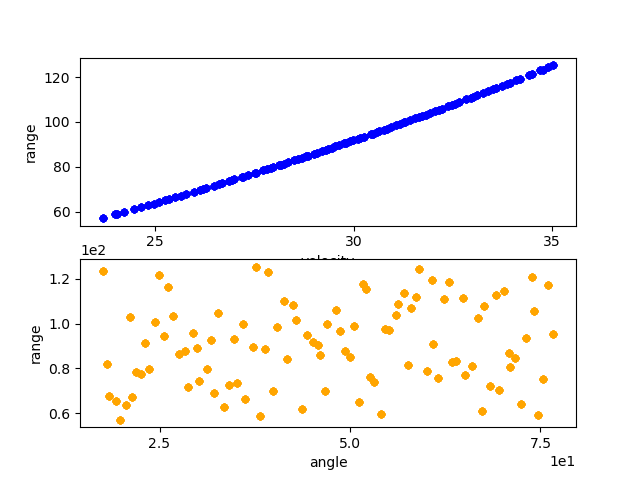
\includegraphics[scale=0.7]{../../tests/framework/user_guide/ForwardSamplingStrategies/gold/RunDir/Stratified/1-historyPlot_scatter-scatter.png}
  \caption{Plot of the histories generated by the Stratified sampling.}
  \label{fig:historiesStratifiedPlotScatter}
 \end{figure}
 %%%%%%%%%%%%%%%%%%%%%%%%%%%%%%%%%%%%%%%%%%%%%%%%%%%%%%%%%%
  In this block, both the Out-Stream types are constructed:
  \begin{itemize}
    \item \textit{Print}:
     \begin{itemize}
       \item named ``samples'' connected with the \textit{DataObjects} \textbf{Entity} ``samples''
                (\xmlNode{source})
       \item named ``histories'' connected with the \textit{DataObjects} \textbf{Entity} ``histories'' (\xmlNode{source}).
     \end{itemize}
      When these objects get used, all the information contained in the
      linked  \textit{DataObjects} are going
    to be exported in CSV files (\xmlNode{type}).
    \item \textit{Plot}:
    \begin{itemize}
      \item named ``historiesPlot'' connected with the  \textit{DataObjects}
      \textbf{Entity} ``histories''.  This plot shows the variable $range$ with respect to the input variables $velocity$ and $angle$.
      \item named ``samplesPlot3D'' connected with the
      \textit{DataObjects} \textbf{Entity} ``samples''. This plot shows the variables $range,time$ with respect to the input variables $velocity$ and $angle$.
    \end{itemize}
  \end{itemize}
   \item \textbf{\textit{Steps}}:
     \xmlExample{framework/user_guide/ForwardSamplingStrategies/forwardSamplingStratified.xml}{Steps}
 %%%%%%%%%%%%%%%%%%%%%%%%%%%%%%%%%%%%%%%%%%%%%%%%%%%%%%%%%%
 %figure samples
 \begin{figure}[h!]
  \centering
  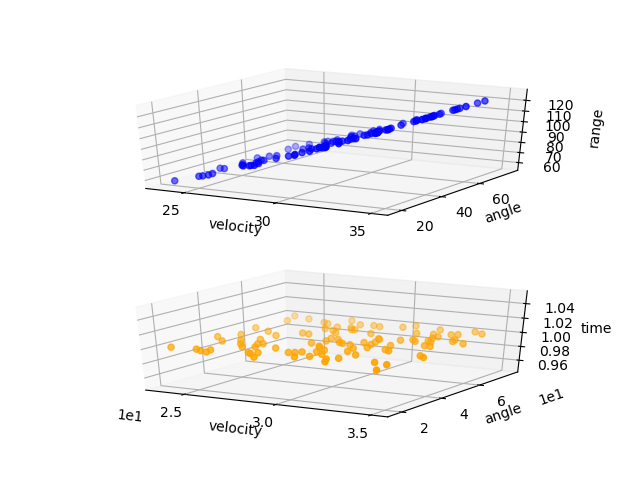
\includegraphics[scale=0.7]{../../tests/framework/user_guide/ForwardSamplingStrategies/gold/RunDir/Stratified/1-samplesPlot3D_scatter-scatter.png}
  \caption{Plot of the samples generated by the Stratified sampling.}
  \label{fig:samplesStratifiedPlotLine}
 \end{figure}
 %%%%%%%%%%%%%%%%%%%%%%%%%%%%%%%%%%%%%%%%%%%%%%%%%%%%%%%%%%
   Finally, all the previously defined \textbf{Entities} can be combined in
   the \xmlNode{Steps} block. As inferable,
   two \xmlNode{Steps} have been inputted:
   \begin{itemize}
     \item \xmlNode{MultiRun} named ``sample'', used to run the multiple
     instances of the driven code and
     collect the outputs in the two \textit{DataObjects}. As it can be
     seen, the \xmlNode{Sampler} is inputted to communicate to the
     \textit{Step} that the driven code needs to
     be perturbed through the Stratified sampling.
     \item  \xmlNode{IOStep} named ``writeHistories'', used to 1) dump
     the ``histories'' and ``samples'' \textit{DataObjects}
     \textbf{Entity} in a CSV file and 2) plot the data in the PNG file and
     on the screen.
   \end{itemize}
\end{enumerate}
 As previously mentioned, Figures~\ref{fig:historiesStratifiedPlotScatter} and ~\ref{fig:samplesStratifiedPlotScatter}  display the report generated by RAVEN.

%%%%%%%%%%%%%%%%%%%%%%%%%

\subsection{Sparse Grid Collocation sampling through RAVEN}
\label{sub:SGcsamplingExample}
The Sparse Grid Collocation sampler represents an advanced methodology to perform Uncertainty Quantification. They aim
to explore the input space leveraging the information contained in the associated probability density functions. It builds on generic Grid sampling by selecting evaluation points based on characteristic quadratures as part of stochastic collocation for generalized polynomial chaos uncertainty quantification. In collocation an N-D grid is constructed, with each uncertain variable providing an axis. Along each axis, the points of evaluation correspond to quadrature points necessary to integrate polynomials. In the simplest (and most naive) case, a N-D tensor product of all possible combinations of points from each dimension’s quadrature is constructed as sampling points. The number of necessary samples can be reduced by employing Smolyak-like sparse grid algorithms, which use reduced combinations of polynomial orders to reduce the necessary sampling space.
\\The goals of this section are about learning how to:
 \begin{enumerate}
   \item Set up a Sparse Grid Collocation sampling for the construction of a suitable surrogate model of a driven code
   \item Construct a GaussPolynomialRom surrogate model (training stage)
   \item Use the constructed GaussPolynomialRom surrogate model instead of the driven code.
\end{enumerate}
To accomplish these tasks, the following RAVEN \textbf{Entities} (XML blocks in the input files) need to be defined:
\begin{enumerate}
   \item \textbf{\textit{RunInfo}}:
     \xmlExample{framework/user_guide/ForwardSamplingStrategies/forwardSamplingSparseGrid.xml}{RunInfo}
   AThe \textit{RunInfo} \textbf{Entity} is intended to set up the analysis  that the user wants to perform. The steps listed in (\xmlNode{Sequence}) are going to be sequentially run using the number of processors specified in  (\xmlNode{batchSize}).  The first two steps build the ROM
   (\xmlString{sample}, \xmlString{train}), the next two validate
   the ROM against the original Code Model (\xmlString{validateModel}, \xmlString{validateROM}),
   \xmlString{rom\_stats} stores ROM-related information into DataObject,
   and the last two produce plots and print data (\xmlString{output\_print}, \xmlString{output\_plot}).
   \item \textbf{\textit{Models}}:
     \xmlExample{framework/user_guide/ForwardSamplingStrategies/forwardSamplingSparseGrid.xml}{Models}
 The goal of this example is the generation of a \text{GaussPolynomialRom}
 for subsequent usage.  In addition to the previously explained External model, the ROM of type \textit{GaussPolynomialRom} is specified here. The ROM is generated through a Sparse Grid Collocation sampling strategy. Note that the \xmlNode{Interpolation} nodes are not required, but are included for the sake of demonstration.
   \item \textbf{\textit{Distributions}}:
     \xmlExample{framework/user_guide/ForwardSamplingStrategies/forwardSamplingSparseGrid.xml}{Distributions}
  In the Distributions XML section, the stochastic model for the
  uncertainties  treated by the Sparse Grid Collocation sampling are reported. In
  this case two distributions are defined:
  \begin{itemize}
    \item $vel\_dist \sim \mathbb{N}(30,5)$, used to model the uncertainties
    associated with  the \textit{velocity};
    \item  $angle\_dist \sim \mathbb{U}(5,85)$,  used to
    model the uncertainties associated with the \textit{angle}.
  \end{itemize}
   \item \textbf{\textit{Samplers}}:
     \xmlExample[rom,ROM,SparseGridCollocation,MonteCarlo]{framework/user_guide/ForwardSamplingStrategies/forwardSamplingSparseGrid.xml}{Samplers}
  In order to employ the Sparse Grid Collocation sampling strategy, a
  \xmlNode{SparseGridCollocation} node needs to be defined.
  As can be  seen from above, each variable is associated with a different distribution,
  defined in the  \xmlNode{Distributions} block.
  In addition, the \textit{GaussPolynomialRom} \xmlNode{ROM} is linked to the \xmlNode{SparseGridCollocation} sampler.  Because this sampler is used exclusively to build the ROM, some of the parameters of the ROM are  needed by the sampler, and this connection makes that communication possible.  The setting of this ROM (e.g. polynomial order, Index set method, etc.) determines how the Stochastic Collocation Method is employed.

  Additionally, a \xmlNode{MonteCarlo} sampler is set up for validating the ROM against the original Code.  The random number generation seed (\xmlNode{initialSeed}) is specified and set to reset on each use (\xmlNode{reseedEachIteration}) so that the Monte Carlo sampler can be used to compare the ROM against the  original model.  We use 100 samples (\xmlNode{limit}) to sample the ROM and the model, and then print and plot both data sets to compare them.
   \item \textbf{\textit{DataObjects}}:
     \xmlExample[rom,SparseGridCollocation]{framework/user_guide/ForwardSamplingStrategies/forwardSamplingSparseGrid.xml}{DataObjects}
  In this block, five \textit{DataObjects} are defined:
  1) a PointSet named ``inputPlaceholder'' used as a placeholder input for the ROM sampling step,
  2) a PointSet named ``samplesModel'' to store the Code responses from Monte Carlo samples,
  3) a PointSet named ``samplesROM'' to store the ROM responses from Monte Carlo samples,
  4) a HistorySet named ``histories'' used to collect the samples needed to train the ROM, and
  5) a DataSet named ``rom\_stats'' to store information from the ROM.
 %%%%%%%%%%%%%%%%%%%%%%%%%%%%%%%%%%%%%%%%%%%%%%%%%%%%%%%%%%
 %%%%%%%%%%%%%%%%%%%%%%%%%%%%%%%%%%%%%%%%%%%%%%%%%%%%%%%%%%
 %figure histories
 \begin{figure}[h!]
  \centering
  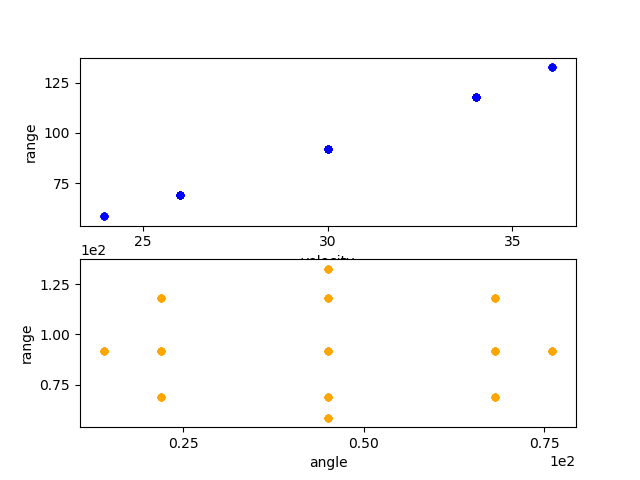
\includegraphics[scale=0.7]{../../tests/framework/user_guide/ForwardSamplingStrategies/gold/RunDir/SparseGrid/1-historyPlot_scatter-scatter.png}
  \caption{Plot of the training samples generated by the SparseGridCollocation sampling for variables $A,B,C,D$.}
  \label{fig:historiesSparseGridPlotScatter}
 \end{figure}
 %%%%%%%%%%%%%%%%%%%%%%%%%%%%%%%%%%%%%%%%%%%%%%%%%%%%%%%%%%
 %%%%%%%%%%%%%%%%%%%%%%%%%%%%%%%%%%%%%%%%%%%%%%%%%%%%%%%%%%
   \item \textbf{\textit{OutStreams}}:
     \xmlExample{framework/user_guide/ForwardSamplingStrategies/forwardSamplingSparseGrid.xml}{OutStreams}
  In this block, the following Out-Stream types are constructed:
  \begin{itemize}
    \item \textit{Print}:
     \begin{itemize}
       \item named ``samplesModel'' connected with the \textit{DataObjects} \textbf{Entity} ``samplesModel''
                (\xmlNode{source})
       \item named ``samplesROM'' connected with the \textit{DataObjects} \textbf{Entity} ``samplesROM''
                (\xmlNode{source})
       \item named ``histories'' connected with the \textit{DataObjects} \textbf{Entity} ``histories'' (\xmlNode{source})
       \item named ``rom\_output'' connected with the \textit{ROM} \textbf{Entity} ``rom'' (\xmlNode{source}).
     \end{itemize}
      When these objects get used, all the information contained in the
      linked  \textit{DataObjects} are going
    to be exported in ether CSV files for DataObjects or XML files for ROMs (\xmlNode{type}).
    \item \textit{Plot}:
    \begin{itemize}
      \item named ``historyPlot'' connected with the  \textit{DataObjects}
      \textbf{Entity} ``histories''.  This plots the
      variable $range$ with respect to the input variables $velocity$ and $angle$.
      \item named ``samplesModelPlot3D'' connected with the
      \textit{DataObjects} \textbf{Entity} ``samplesModel''. This plot will draw the
      variables $range,time$ as Monte Carlo sampled on the Code.
      \item named ``samplesROMPlot3D'' connected with the
      \textit{DataObjects} \textbf{Entity} ``samplesROM''. This plot will draw the
      variables $range,time$ as Monte Carlo sampled on the ROM.
    \end{itemize}
  \end{itemize}
   \item \textbf{\textit{Steps}}:
     \xmlExample[rom,SparseGridCollocation]{framework/user_guide/ForwardSamplingStrategies/forwardSamplingSparseGrid.xml}{Steps}
  %%%%%%%%%%%%%%%%%%%%%%%%%%%%%%%%%%%%%%%%%%%%%%%%%%%%%%%%%%
 %figure samples
 \begin{figure}[h!]
  \centering
  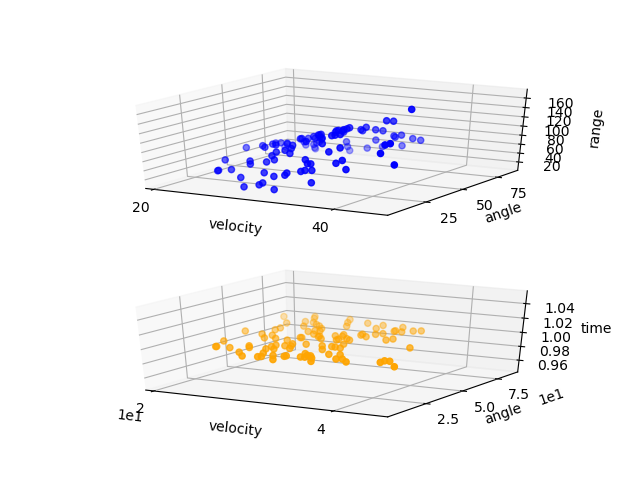
\includegraphics[scale=0.7]{../../tests/framework/user_guide/ForwardSamplingStrategies/gold/RunDir/SparseGrid/1-samplesModelPlot3D_scatter-scatter.png}
  \caption{Plot of validation samples generated by Monte Carlo sampling on the Code.}
  \label{fig:samplesSparseGridPlotModel}
 \end{figure}
 %%%%%%%%%%%%%%%%%%%%%%%%%%%%%%%%%%%%%%%%%%%%%%%%%%%%%%%%%%
   Finally, the previously defined \textbf{Entities} can be combined in
   the \xmlNode{Steps} block.
   The following \xmlNode{Steps} have been defined:
   \begin{itemize}
     \item \xmlNode{MultiRun} named ``sample'', used to run the training
     samples of the driven code and
     collect the outputs in the \textit{DataObjects}.
     The \xmlNode{Sampler} is specified to communicate to the
     \textit{Step} that the driven code needs to
     be sampled through the Sparse Grid Collocation sampling strategy;
     \item \xmlNode{RomTrainer} named ``train'', used to train (i.e.,
     construct) the GaussPolynomial ROM. This step is essential if the
     user want to use the ROM in later steps;
     \item \xmlNode{MultiRun} named ``sampleModel'', used to run the
     Monte Carlo perturbed samples of the original Model for use in verification.  The results are
     collected in the \textit{samplesModel} \textit{DataObjects}.
     \item \xmlNode{MultiRun} named ``sampleROM'', used to run the
     Monte Carlo perturbed samples of the previously constructed ROM for use in verificaiton.  The results are
     collected in the \textit{samplesROM} \textit{DataObjects}.
     \item \xmlNode{IOStep} named ``rom\_stas'', used to dump rom-related information into \textit{DataObject },
     \item  \xmlNode{IOStep} named ``output\_print'', used to dump
     the ``histories'', ``samplesModel'' and ``samplesROM'' \textit{DataObjects}
     \textbf{Entity} in a CSV file,
     \item  \xmlNode{IOStep} named ``output\_plot'', used to
     plot the data and store it in the PNG file and
     on the screen.
   \end{itemize}
\end{enumerate}
 % As previously mentioned, Figure~\ref{fig:historiesSparseGridPlotScatter}
 % shows the evolution of the outputs $A,B,C,D$ under uncertainties.
 % Figures~\ref{fig:samplesSparseGridPlotModel} and
 % \ref{fig:samplesROMSparseGridPlot} show the final responses
 % of the sampling employed using the driven code and the ROM,
 % respectively. 
 As it can be seen, the constructed ROM can accurately
 represent the response of the driven code. This example shows the
 potential of reduced order modeling, in general, and of the
 \textit{GaussPolynomialRom}, in particular.

  %%%%%%%%%%%%%%%%%%%%%%%%%%%%%%%%%%%%%%%%%%%%%%%%%%%%%%%%%%
 %figure samples
 \begin{figure}[h!]
  \centering
  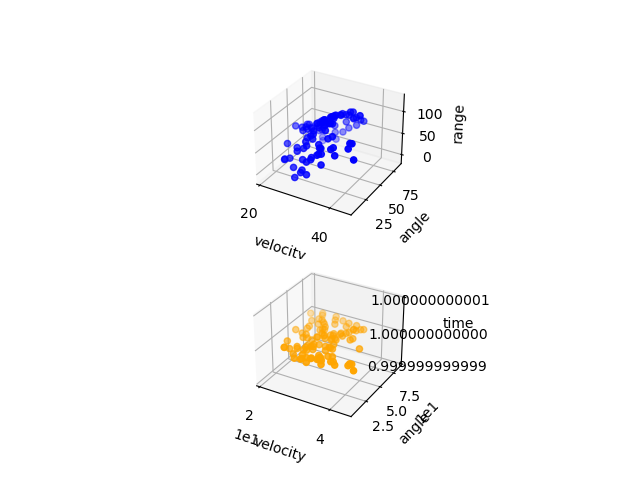
\includegraphics[scale=0.7]{../../tests/framework/user_guide/ForwardSamplingStrategies/gold/RunDir/SparseGrid/1-samplesROMPlot3D_scatter-scatter.png}
  \caption{Plot of validation samples generated by Monte Carlo sampling on the ROM.}
  \label{fig:samplesROMSparseGridPlot}
 \end{figure}
 %%%%%%%%%%%%%%%%%%%%%%%%%%%%%%%%%%%%%%%%%%%%%%%%%%%%%%%%%%








